
\documentclass[12pt]{article}

\usepackage[utf8]{inputenc}
\usepackage[bulgarian]{babel}
\usepackage{graphicx}
\usepackage{sidecap}  %required for side captions
\usepackage{amssymb}
\usepackage{amsmath}
\usepackage{hyperref}
\usepackage{commath}  
\usepackage[top=1.3in, bottom=1.5in, left=1.3in, right=1.3in]{geometry}

\begin{document}
	\begin{center}
        \LARGE{\textbf{Тема: ViZTranZ - превод на обекти от изображение}}
        
        \bigskip
        \Large{Предмет: Приложно-програмни интерфейси за работа с облачни архитектури с Амазон Уеб Услуги (AWS)}
        
        \medskip
        \Large{Изготвил: Симеон Христов, фн: 71845, имейл: s.e.hristov99@gmail.com}
        
        \medskip
        \Large{Лектор: доц. д-р Милен Петров, година: 2022}
        
        \bigskip
	\end{center}
    
    
  %  \newpage
    \tableofcontents
    \bigskip
    \bigskip
    \newpage
  
\section{Условие} 

\noindent ViZTranZ е уеб приложение, което позволява на потребител да прикачи снимка и да получи превод на обектите, разпознати в тази снимка.

\section{Въведение}

\noindent Приема се, че преводът винаги се случва от английски към някой от езиците български, немски и руски. Превеждат се етикетите на първите 10 разпознати обекта с най-голяма увереност. Възможно е да не бъдат разпознати обекти в снимката, при което се извежда подходящо съобщение на потребителя.

\noindent В странично (ляво) меню се предлагат двата начина на работа с приложението - с използване услугите на AWS (наричан в приложението "AWS") и без използване услугите на AWS (наричан в приложението "Local"). По подразбиране е избран "Local".

\noindent Начинът на работа се описва с тези стъпки:
\begin{enumerate}
    \item Система показва меню, от което може да бъде прикачена снимка.
    \item Потребителят прикачва (точно една) снимка.
    \item Система показва меню, от което може да бъдат избрани езиците, към които да бъдат преведени разпознатите обекти. Поддържани езици са български, немски и руски. По подразбиране е избран български. Необходимо е да бъде избран поне един език, за да продължи процесът.
    \item Потребителят избира поне един език.
    \item Системата показва бутон Translate, след натискането на който започва процесът по разпознаване на обектите от снимката и преводът на тяхните етикети.
    \item Потребителят натиска появилия се (най-отдолу) бутон.
    \item В зависимост от начина на работа на приложението се преминава през процеса на разпознаване на обектите от снимката и техния превод.
    \item Системата получава резултатите от превода на етикетите на разпознатите обекти (за всички езици).
    \item Системата показва на потребителя графика (тип бар диаграма), в която по абсцисата са нанесени вероятностите за съществуването на разпознатите обекти в снимката, а по ординатата - преводът на обектите, заедно с етикета на английски.
    \item Потребителят може да избере различни езици, при което резултати ще се изведат мигновенно, т.к. те са налични в паметта, отделена за програмата. По този начин се избягва повторно качване на снимката и задействане на процеса.
\end{enumerate}

\section{Теория}

\noindent В зависимост от начина на работа тук са разгледани техническите детайли по време на процеса по разпознаване на обекти и превод на техните етикети.

\subsection{Работа в режим AWS}

\noindent Когато потребителят натисне бутона Translate, снимката бива качена в предварително създадена база от данни, реализирана в S3. При всяко качване на обект в тази база се задейства чрез тригер ламбда функция. В нея се извлича най-скорошно качената снимка. Тя се подава на Rekognition, откъдето се получава речник с информация за разпознатите обекти. От този речник се извличат етикетите на разпознатите обекти и увереността на модела, че те съществуват в снимката. Всеки етикет (поотделно) се предава на Translate и за трите езика. Преводите се конкатенират със списъка от един елемент - увереността. По този начин се получава речник с ключове - символни низове, представляващи етикетите на разпознатите обекти (на английски език), и стойности - хетерогенни списъци, чиито първи елементи са увереностите на модела, а следващите три са символни низове, представляващи превода на ключа в трите езика. Този речник се записва в друга база от данни, отново в S3, откъдето е (поименно) достъпена в приложението. Резултатите се съхраняват под формата на json. След изтегляне в приложението резултатите се трансформират в таблица (pandas dataframe) и се визуализират под формата на bar диаграма, създадена чрез plotly.

\subsection{Работа в режим Local}

\noindent В този режим се използват две основни технологии - Tensorflow и Hugging Face Transformers. Tensorflow е рамка за създаване на невронни мрежи. В случая се използва вече създадена и тренирана невронна мрежа за разпознаване на обекти в снимки - mobilenetv2, чиито тегла предварително са изтеглят по време на процесът по подготвяне на приложението. От нея отново се взимат разпознатите етикети и увереността в тях. С цел бързодействие избраният модел не е толкова добър в разпознаването на обекти и поради тази причина се наблюдават по-слаби резултати. Понеже няма модел (невронна мрежа), който е достатъчно малък и бърз, за превод от английски към трите езика на веднъж, етикетите се превеждат чрез три модела. Моделът opus-mt-en-bg се използва за превод от английски към български. Моделът opus-mt-en-ru се използва за превод от английски към руски. Моделът opus-mt-en-de се използва за превод от английски към български.

\section{Използвани технологии}

\subsection{Технологии, свързани с AWS}

\begin{itemize}
    \item \textbf{AWS Identity and Access Management (IAM)} - за създаване на роли за ламбда функцията, както и за достъпът до S3.
    \item \textbf{AWS Cost Explorer} - за създаване на бюджет и сигнализация при надминаването му.
    \item \textbf{Amazon Simple Storage Service (Amazon S3)} - за съхраняване на снимките и резултатите.
    \item \textbf{AWS Lambda} - за мост между S3, Rekognition, и Translate.
    \item \textbf{AWS Rekognition} - за разпознаване на обекти.
    \item \textbf{AWS Translate} - за превод етикетите на обекти.
    \item \textbf{AWS CloudWatch} - за наблюдаване на работата на ламбда функцията.
\end{itemize}

\subsection{Други технологии}

\begin{itemize}
    \item \textbf{Python} - езикът, на който е реализирано приложението.
    \item \textbf{Streamlit} - библиотека на Python, чрез която е създадено уеб приложението.
    \item \textbf{Tensorflow} - за създаване и използване на невронни мрежи. В случая, използвана за разпознаване на обекти от изображение.
    \item \textbf{Hugging Face} - за работа с текст. В случая, използвана за превод етикетите на обекти.
\end{itemize}

\section{Инсталация и настройки}
\noindent\textbf{Стъпка 1.} Отваря се терминал в директорията на приложението.

\medskip

\noindent\textbf{Стъпка 2.} Пуска се файлът setup.sh.

\medskip

\noindent\textbf{Стъпка 3. (Незадължителна)} Ако ще се използва режим на работа AWS е нужно да се поставят данни за удостоверяване в копие на .env-example.

\medskip

\noindent\textbf{Стъпка 4.} Пуска се файлът run.sh.

\section{Кратко ръководство за потребителя и примерни данни}

\begin{figure}[!htp]
\centering
    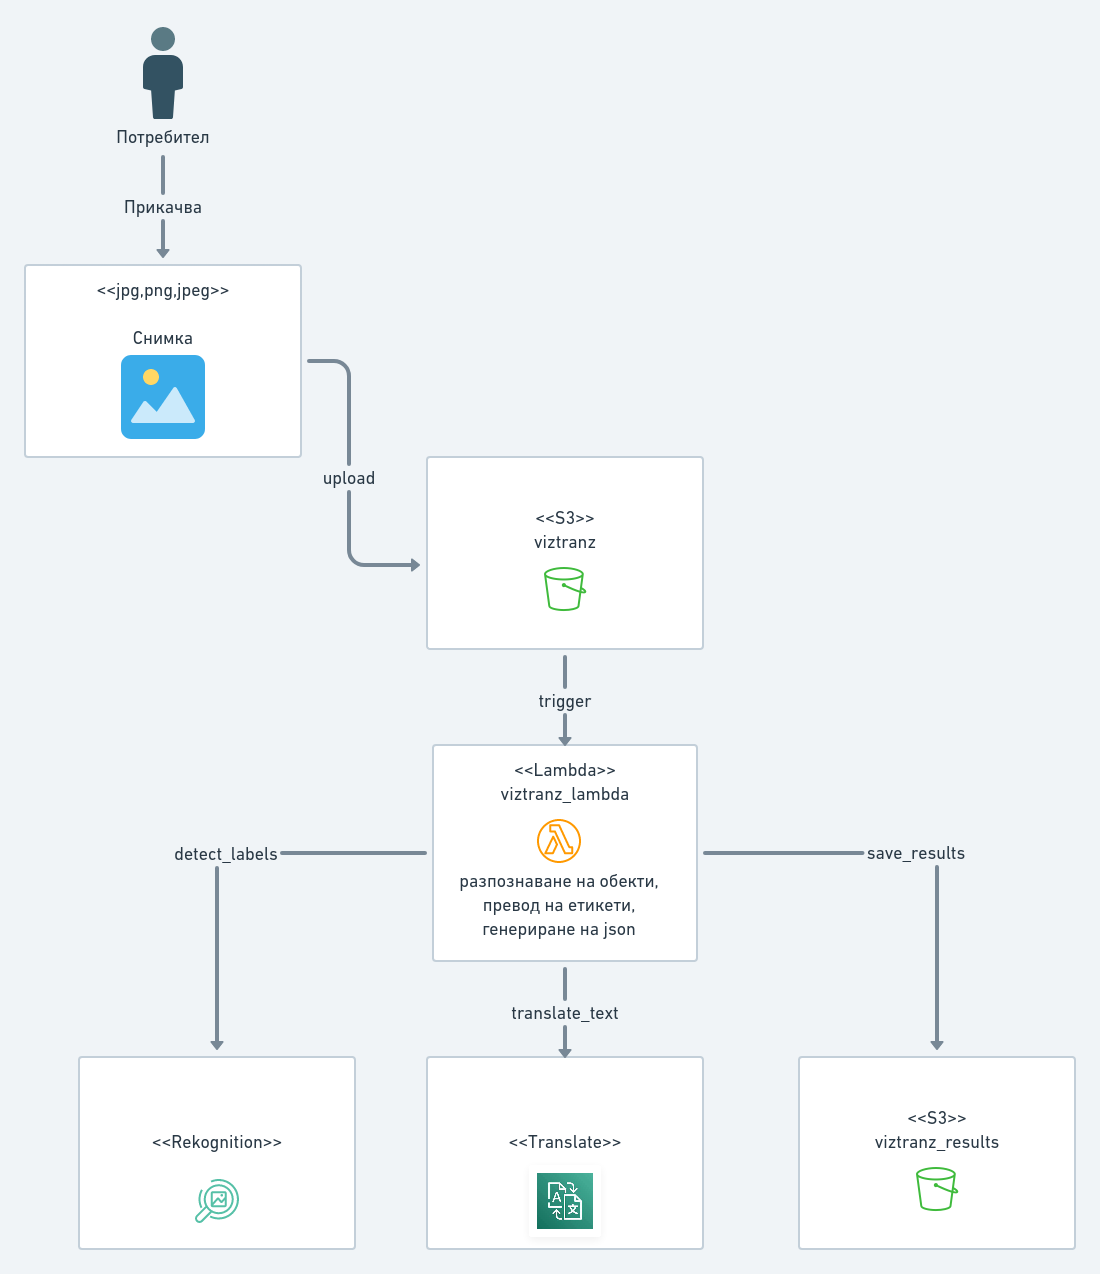
\includegraphics[scale=0.28]{assets/ViZTranZ.png}
  \caption{Структура на услугите, използвани в режим AWS}
\end{figure}

\noindent За да се получат правилно преводи е нужно да се качи снимка, на която има поне един ясно различим обект. Следващите стъпки показват примерна ситуация.

\begin{figure}[!htp]
\centering
    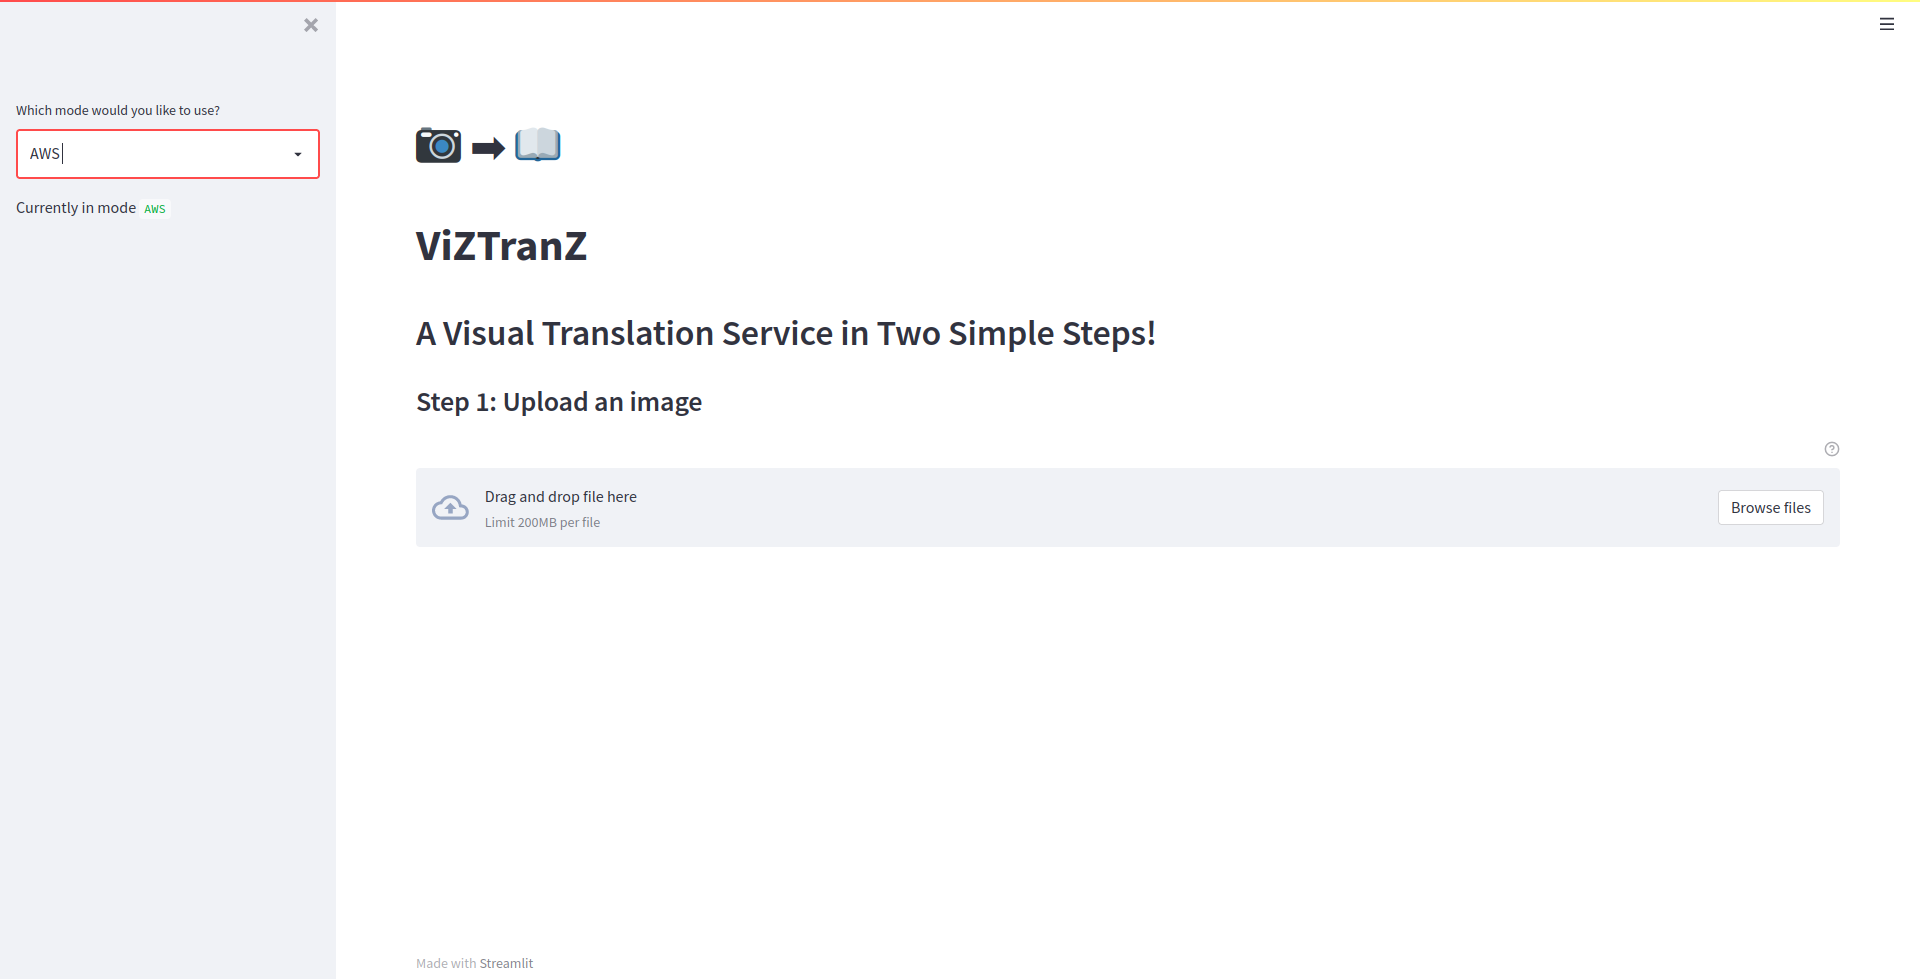
\includegraphics[scale=0.2]{assets/st1.png}
  \caption{\textbf{Стъпка 1.} Избира се AWS от ляво меню.}
\end{figure}

\begin{figure}[!htp]
\centering
    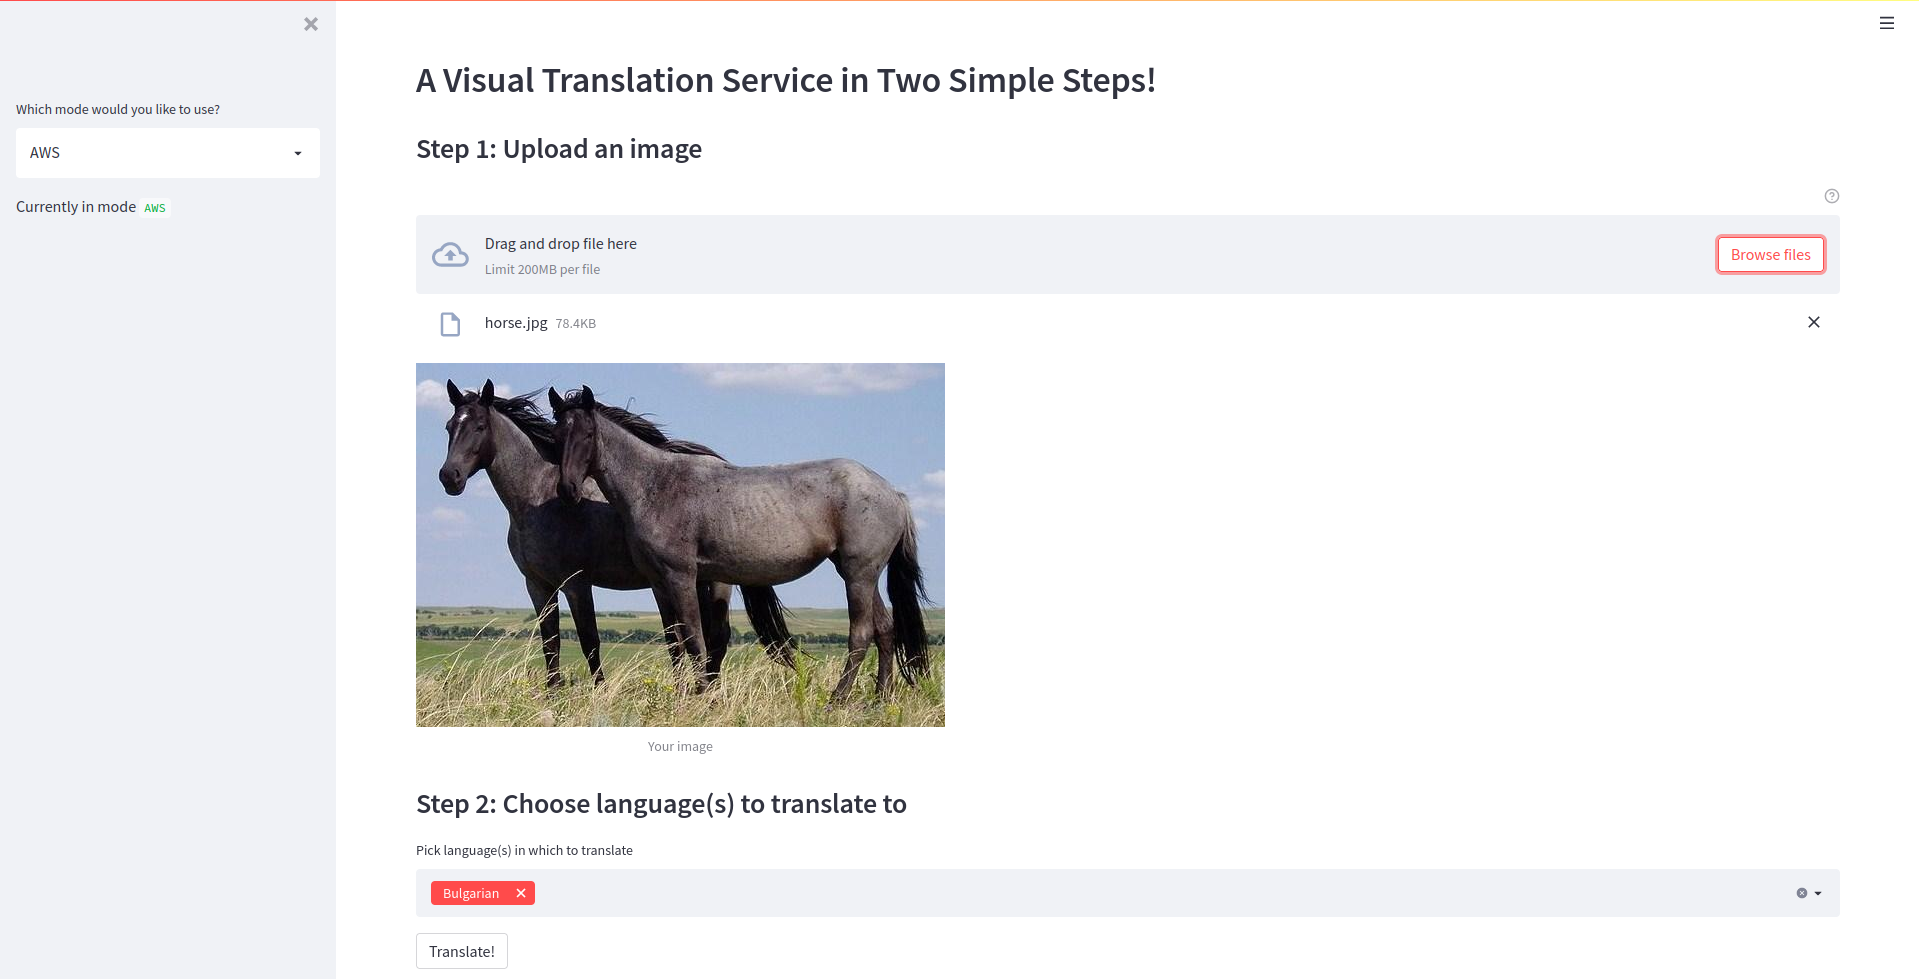
\includegraphics[scale=0.2]{assets/st2.png}
  \caption{\textbf{Стъпка 2.} Прикачва се снимка.}
\end{figure}

\begin{figure}[!htp]
\centering
    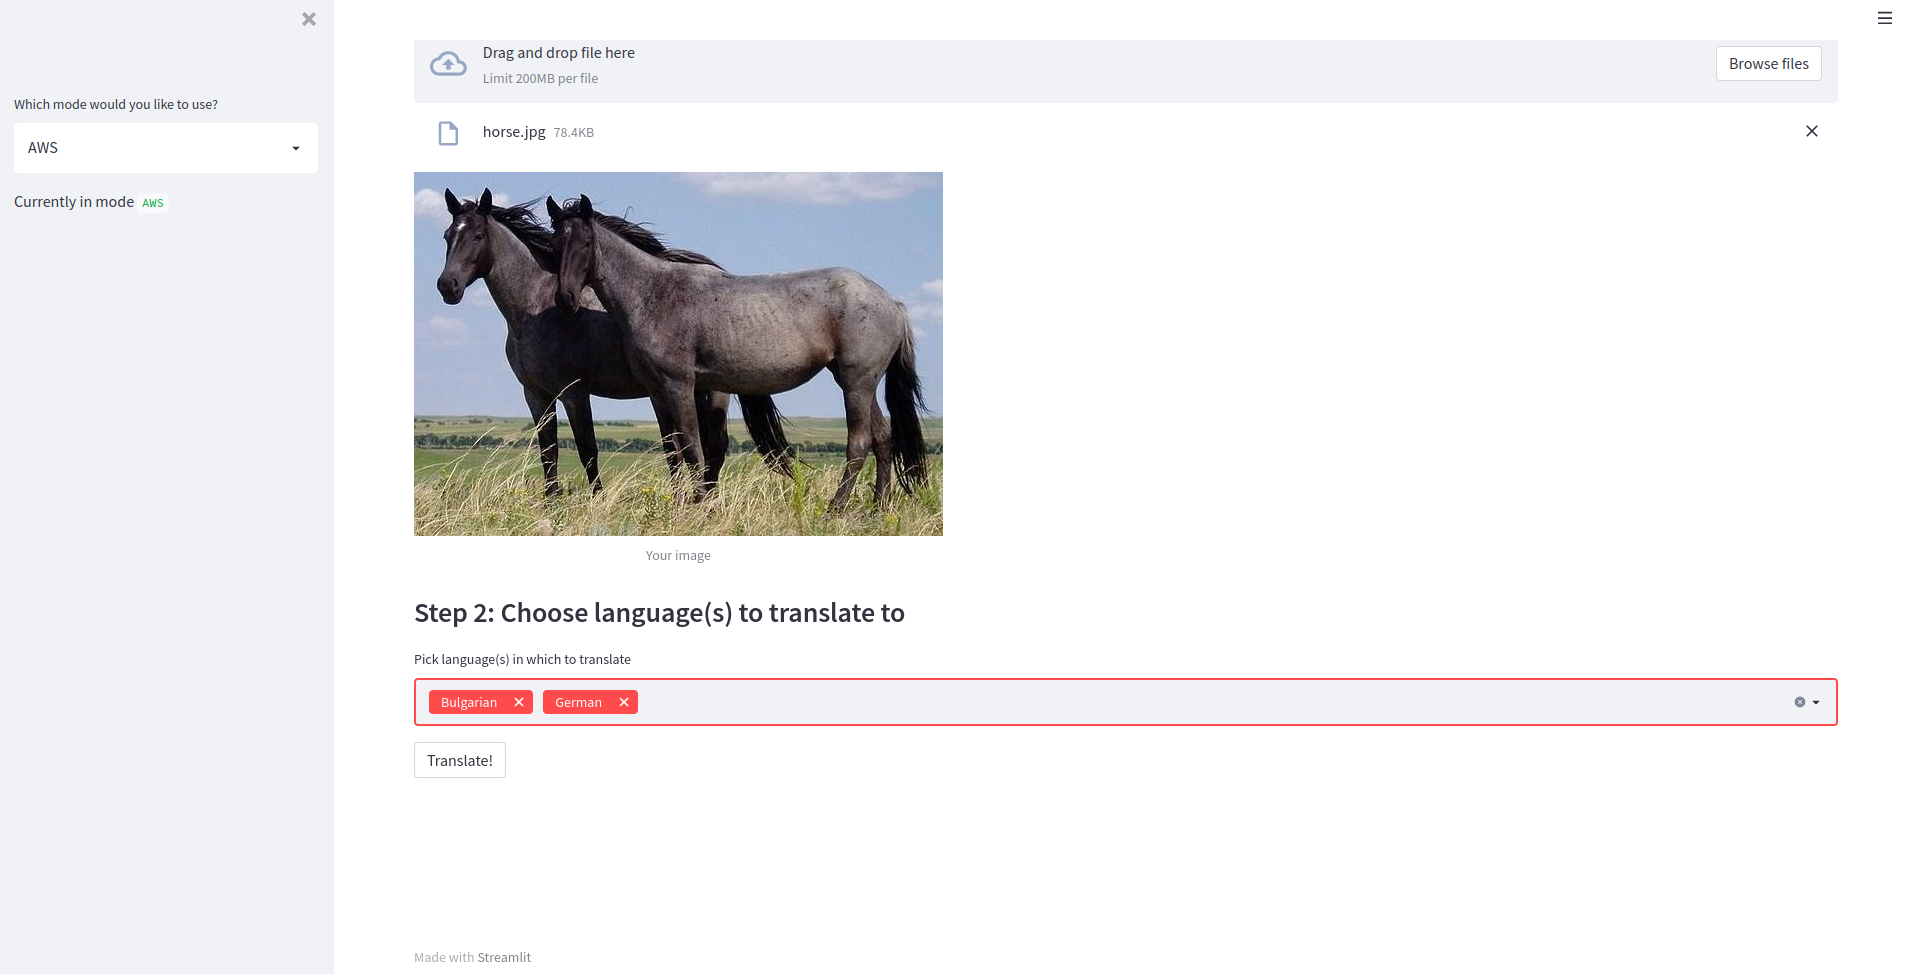
\includegraphics[scale=0.2]{assets/st3.png}
  \caption{\textbf{Стъпка 3.} Избират се езици за превод.}
\end{figure}

\begin{figure}[!htp]
\centering
    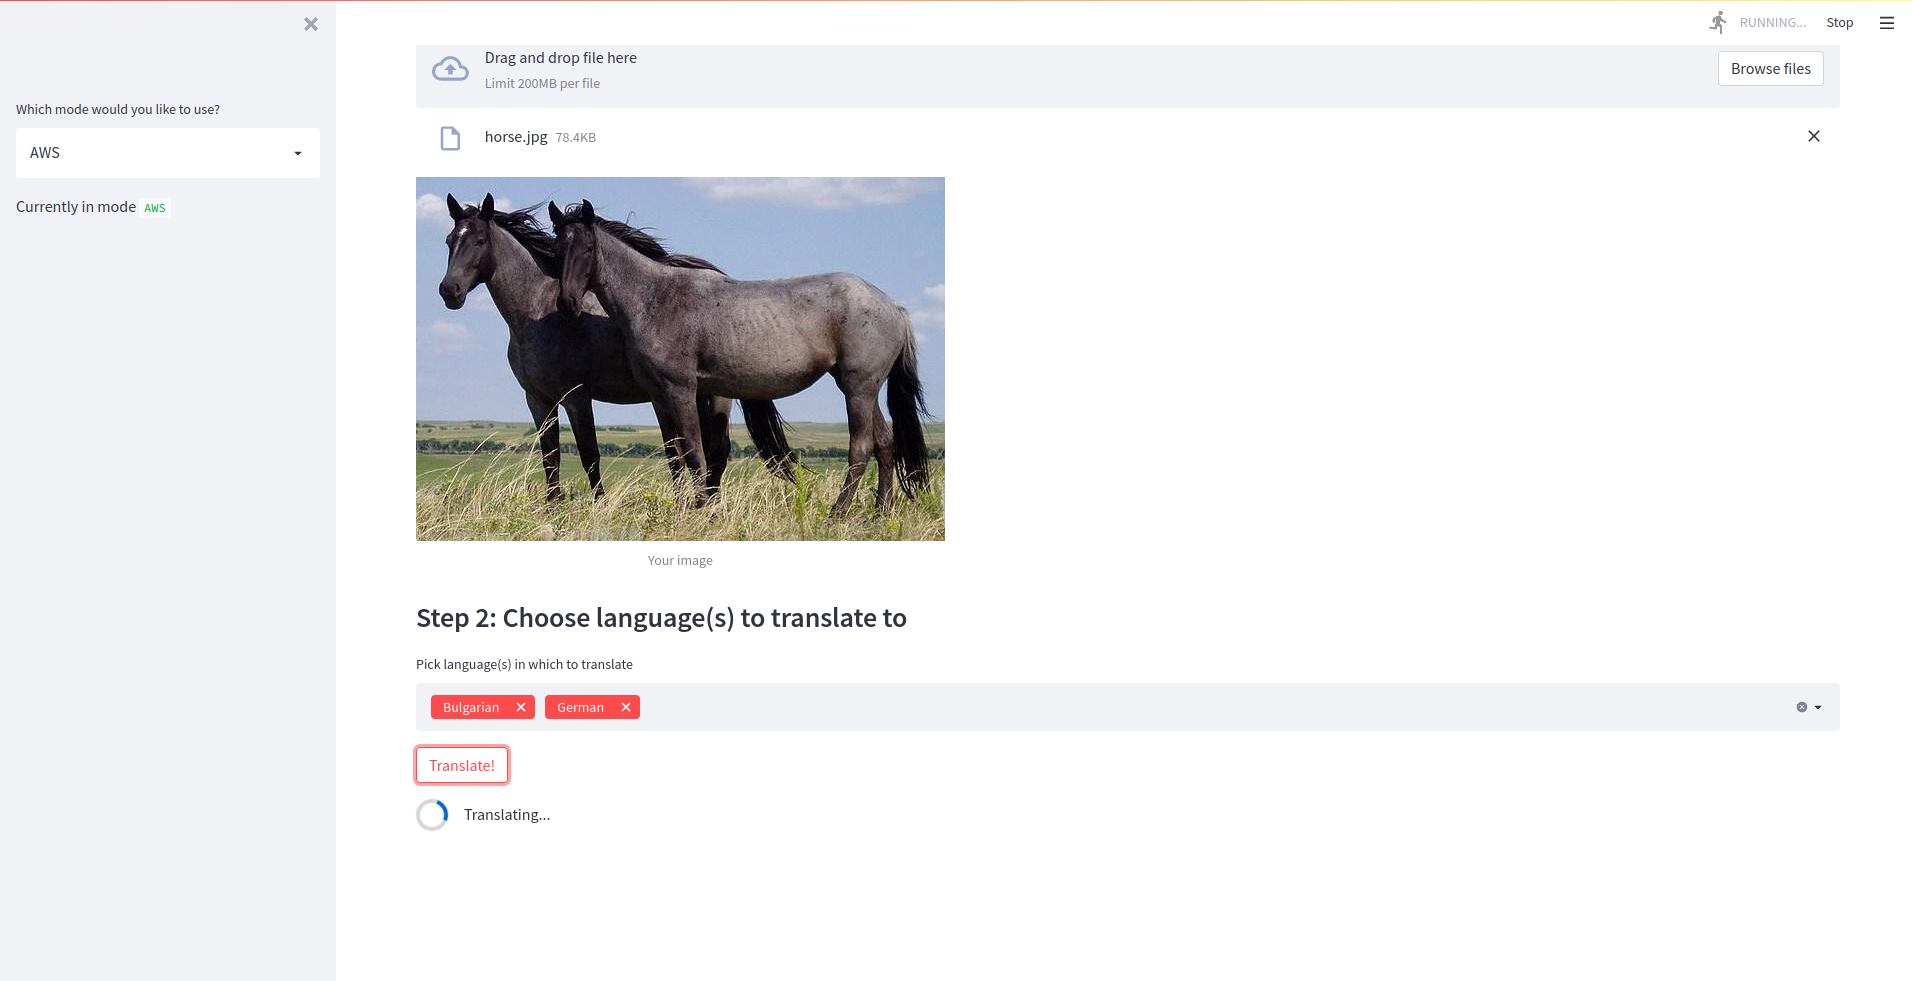
\includegraphics[scale=0.2]{assets/st4.png}
  \caption{\textbf{Стъпка 4.} Натиска се бутон Translate.}
\end{figure}

\noindent \textbf{} 

\begin{figure}[!htp]
\centering
    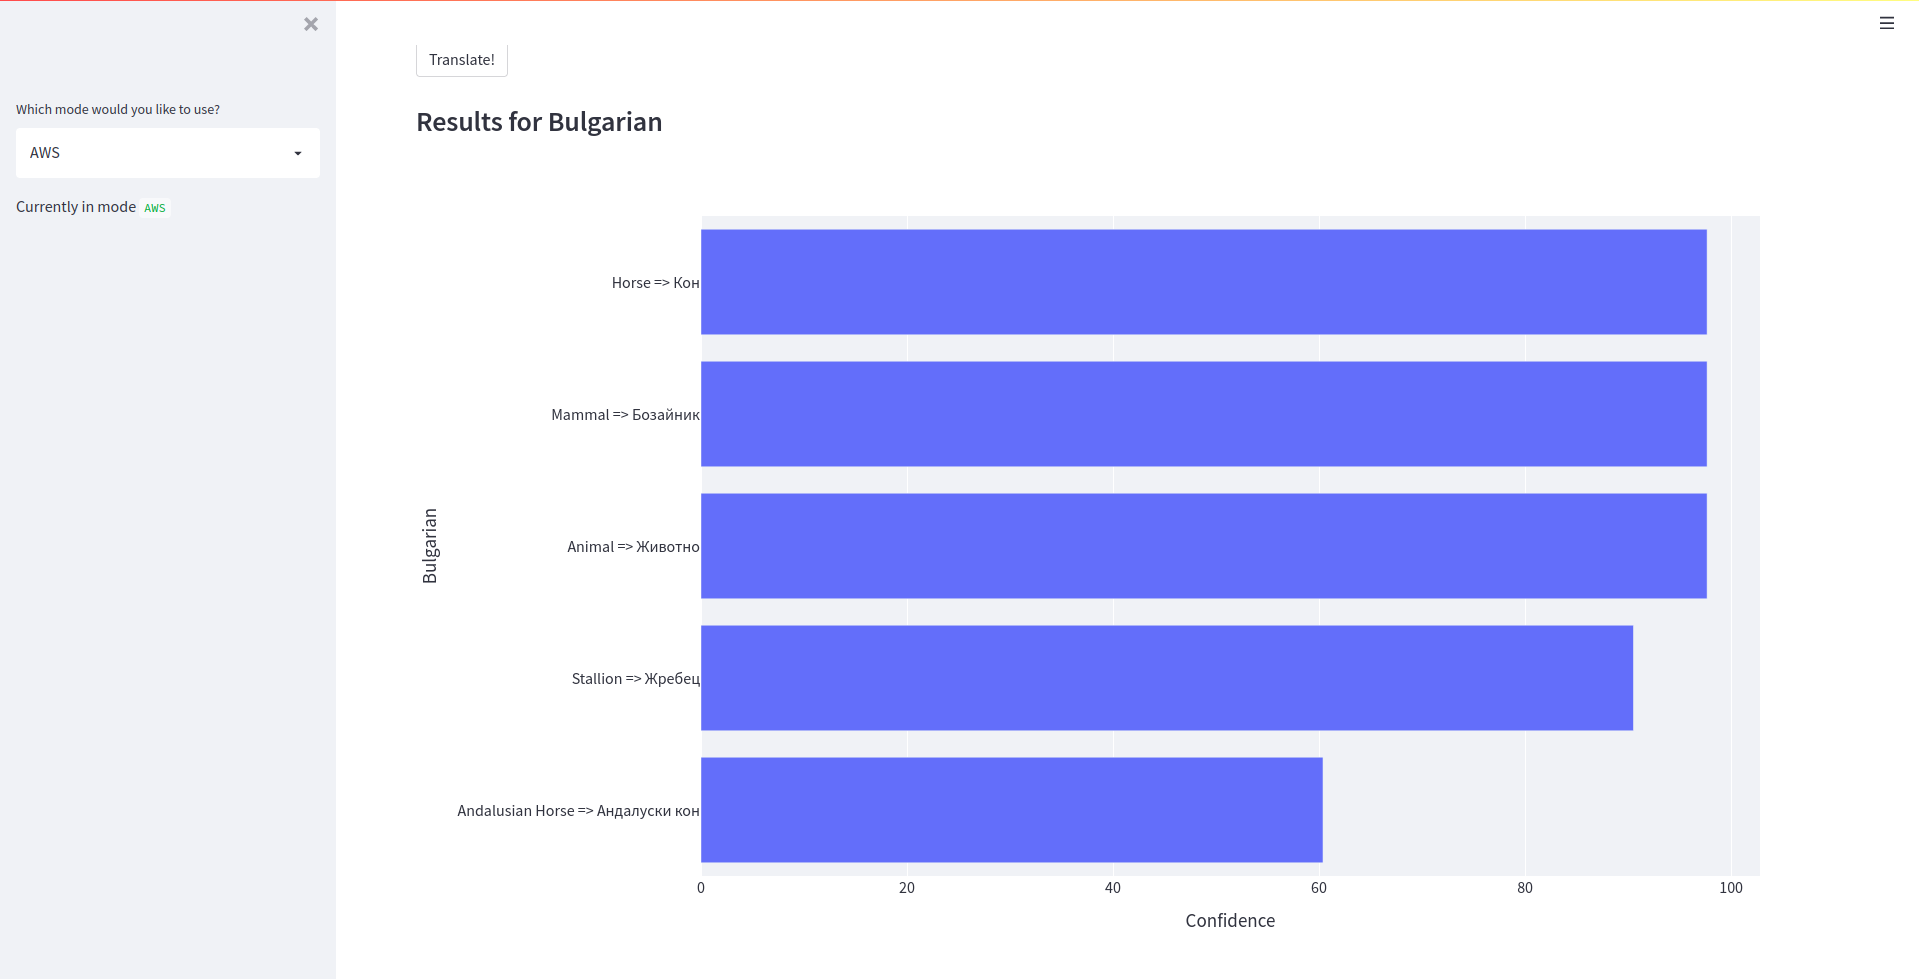
\includegraphics[scale=0.2]{assets/st5_1.png}
  \caption{\textbf{Стъпка 5.1.} Наблюдават се резултати за български}
\end{figure}

\begin{figure}[!htp]
\centering
    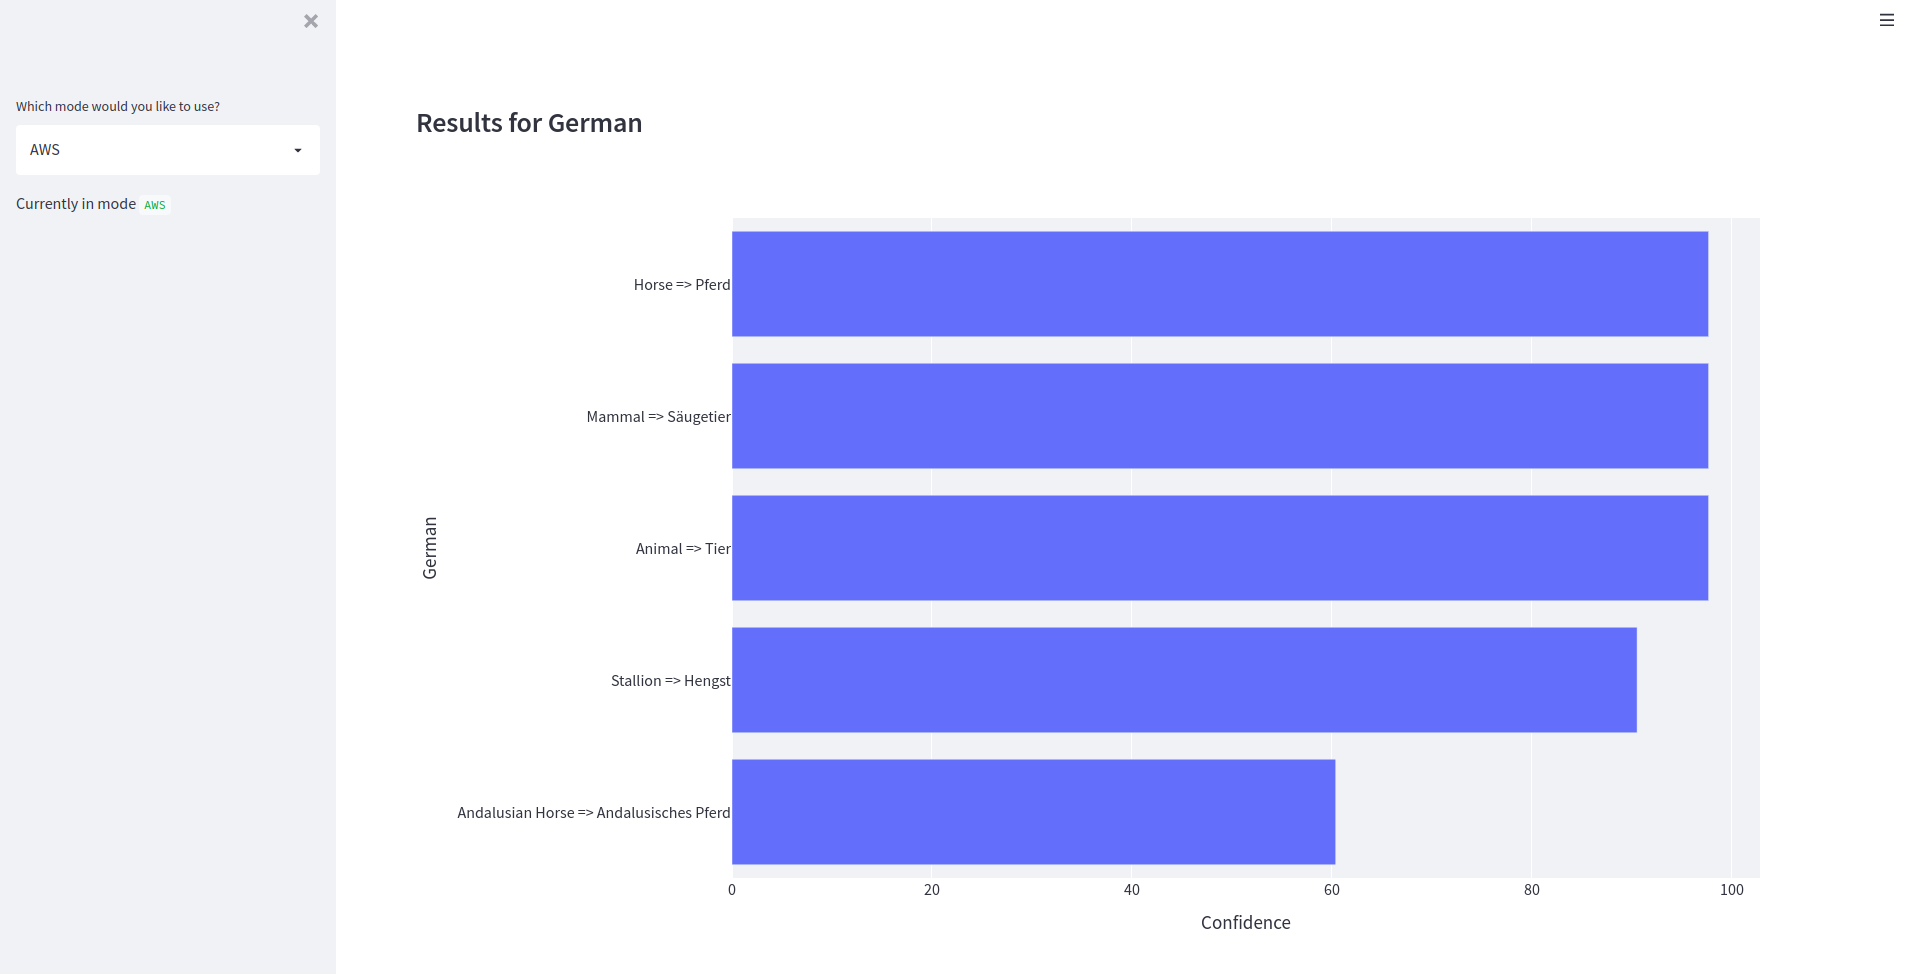
\includegraphics[scale=0.2]{assets/st5_2.png}
  \caption{\textbf{Стъпка 5.2.} Наблюдават се резултати за немски}
\end{figure}

\section{Описание на програмния код}

Приложението се състои от един пакет - viztranz и един външен файл (модул), който управлява приложението - app.py.

\subsection{Файл app.py}

\noindent Основният файл, който генерира уеб съдържанието и чрез който се управлява цялото приложение. Разделен е на три части - заглавна част, странично меню и главно меню. В заглавната част се поставя настройка за използване на режим широк екран, при който всяко поле (widget) ще заема максимална широчина. Поставя се също и икона на страницата, както и заглавие. Те могат да бъдат видяни в табът, отворен от браузъра. С последните три команди се дава заглавие и уточняващ текст, който описва целта на приложението.

\noindent В секцията странично меню се задава selectbox, чрез който потребителят може да избере режим на работа. След промяна на режима на работа, ако са съществували резултати от предишен превод, те ще бъдат изтрити.

\noindent В секцията главно меню се показват различните подменюта. Първо, се показва това за прикачване на файл. Може да прикачен точно един файл. Ако това се случи, снимката се визуализира и потребителят е подканен да избере езици, на които желае да преведе разпознатите обекти. За да се продължи напред, е нужно да бъде избран поне един език. Ако това се случи се показва бутон Translate, при натискането на който, в зависимост от режима на работа, се извикват съответните методи за разпознаване на обекти и превод на тяхните етикети. Понеже тези процеси отнемат време, се визуализира и spinner, който гарантира, че приложението работи. Когато бъдат получени резултатите, те се запазват в паметта на програмата и се поставят в pandas dataframe, чрез който лесно могат да се визуализират под формата на хоризонтална bar диаграма. 

\subsection{Файл constants.py}

\noindent Тук се съхраняват глобални променливи и константи. Константата SUPPORTED-LANGS задава поддържаните от приложението езици за превод. Редът е от значение е нови езици е нужно да бъдат добавяни в края. Променливата results съхранява получените резултати след превод. Чрез нея се избягва повторно задействане на процедурата по разпознаване и превод. С други думи, ако потребителят реши да получи други преводи за същата снимка ще се използва тази променлива. Текущият режим на работа се записва в променливата mode. Константата MODULE-HANDLE съхранява пътят до директорията, съхраняваща моделът, използван от Tensorflow за разпознаване на обекти в режим на работа Local. Функцията get-sample-results връща примерни резултати. Би се използвала за тестване, без да е нужно преминаване през AWS.

\subsection{Файл helper.py}

\noindent Съхранява помощни функции, използвани в основния файл (app.py). 

\noindent Функцията toggle-results затрива текущо запазените резултати за превод. Тя се извиква, когато се качи нова снимки или се избере друг режим на работа.

\noindent Функцията get-upl-file показва меня за прикачване на снимка и връща прикачената снимка, запазена в паметта.

\noindent Функцията get-langs показва меню за избор на език и връща избраните езици под формата на списък от символни низове.

\noindent Функцията build-chart създава pandas dataframe и го визуализира под формата на bar диаграма. По абсцисата се представя увереността на модела, че такъв обект съществува в снимката, а по ординатата - превод на съответния етикет.

\noindent Функцията add-translations добавя преводи към разпознатите обекти. Използва се в режим Local. 

\subsection{Файл lambda.py}

Файл, който съхранява кодът на ламбда функцията, дефинирана в AWS.

\subsection{Файл s3-manager.py}

Съхранява кодът, използван за работа с S3.

\noindent Понеже за свързване с S3 са нужен акаунт, първите неща, които се зареждат в този файл са двата ключа, необходими за оторизация и името на базата от данни, в която ще бъде записан резултатът от превода. След това зареждане се дефинира и клиентът, който ще "общува" с AWS.

\noindent Функцията gen-name генерира име на файла, който ще бъде записан в базата от данни, която ще задейства ламбда функцията, и база от данни, в която ще бъдат записани резултати. Това е необходимо, т.к. няма достъп до самата ламбда и файловете се разпознават само по тяхното име.

\noindent Функцията upload прикачва изображението в S3.

\noindent Функцията get-results извлича резултатите от базата от данни, която ги съхранява.

\subsection{Файл tf-od.py}
\noindent Тук се съхранява кодът, който извършва разпознавате на обекти в режим на работа Local.

\noindent Променливата detector съхранява използвания модел.

\noindent Функцията run-detector извършва разпознаването на обекти.

\subsection{Файл translation.py}

\noindent Тук се съхранява кодът, който извършва превод на етикетите на разпознатите обекти в режим на работа Local.

\noindent Променливите tr-ru, tr-de, и tr-bg са инстанции на трите модела за превод.

\noindent Речникът translators съхранява описаните по-горе инстанции на класовете.

\noindent Функцията translate използва даден модел за превод на текст и връща превода.

\section{Приноси на студента, ограничения и възможности за бъдещо развитие}

Създадено е приложение, което може да бъде използвано за превод на обекти от снимки в реално време. Подходящо е за деца, които опознават света, и учат чужди езици.

\medskip

\noindent Към момента има ограничения в точността на моделите в режим Local. Възможно е получаване на грешни резултати с тях. Второто ограничение е в поддържаният набор езици.

\medskip

\noindent В бъдеще е възможно да се добавят други езици, както и да се визуализират преводите не в bar chart, а директно върху изображението, като се използват ограждащите кутии (bounding box), които се връщат от AWS Rekognition по време на разпознаването на обекти. Също така може да се използват двете бази от данни в S3 за анализ на начина, по който се използва приложението (какви снимки се качват, кога има най-много трафик и т.н.) с цел неговото подобряване.

\section{Какво научих}

Научих се как да използвам изброените по-горе услуги, предоставени от AWS. Научих се как да ги интегрирам в реално приложение. Усъвършенствах познанията си по Python и Streamlit.

\section{Списък с фигури}

\listoffigures

\section{Използвани източници}

\noindent\href{https://docs.aws.amazon.com/lambda/?id=docs_gateway}{[1] AWS Lambda Documentation}
 
\medskip

\noindent\href{https://docs.aws.amazon.com/s3/?id=docs_gateway}{[2] Amazon Simple Storage Service Documentation}
 
\medskip

\noindent\href{https://docs.aws.amazon.com/rekognition/?id=docs_gateway}{[3] Amazon Rekognition Documentation}
 
\medskip

\noindent\href{https://docs.aws.amazon.com/translate/?id=docs_gateway}{[4] Amazon Translate Documentation}
 
\medskip

\noindent\href{https://boto3.amazonaws.com/v1/documentation/api/latest/index.html}{[5] Boto3 documentation}
 
\medskip

\noindent\href{https://docs.streamlit.io/}{[6] Streamlit documentation}
 
\medskip

\noindent\href{https://www.tensorflow.org/}{[6] Tensorflow documentation}
  
\medskip

\noindent\href{https://tfhub.dev/}{[7] Tensorflow Hub}

\medskip

\noindent\href{https://huggingface.co/Helsinki-NLP/opus-mt-de-bg}{[8] Hugging Face Transformers for Translations: opus-mt-de-bg}

\medskip

\noindent\href{https://huggingface.co/t5-small}{[9] Hugging Face Transformers for Translations: t5-small}

\bigskip

Изготвил: Симеон Христов

\bigskip

Подпис: 

\end{document}